\documentclass[border=2mm]{standalone}
\usepackage{tikz}
\usetikzlibrary{calc,shapes.misc, positioning}

\begin{document}
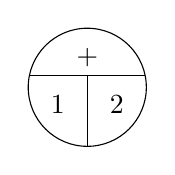
\begin{tikzpicture}
  \newlength{\mywidth}
  \newlength{\myheight}
  \newlength{\mysecantH}
  \setlength{\mywidth}{1.5cm}
  \setlength{\myheight}{\mywidth}
  \setlength{\mysecantH}{0.6\myheight}

  % cerchio
  \draw[rounded corners=\mywidth/2] (0, 0) rectangle (\mywidth, \myheight);
  % separatore orizzontale
  \draw (0.01\mywidth, \mysecantH) -- (0.99\mywidth, \mysecantH);
  % separatore verticale
  \draw (0.5\mywidth, 0) -- (0.5\mywidth, \mysecantH);

  \node (Operatore) at (0.5\mywidth,1.25\mysecantH) {$+$};
  \node (Op1) at (0.25\mywidth,0.35\myheight) {$1$};
  \node (Op2) at (0.75\mywidth,0.35\myheight) {$2$};
  \end{tikzpicture}
\end{document}
